%Version 3.1 December 2024
% See section 11 of the User Manual for version history
%
%%%%%%%%%%%%%%%%%%%%%%%%%%%%%%%%%%%%%%%%%%%%%%%%%%%%%%%%%%%%%%%%%%%%%%
%%                                                                 %%
%% Please do not use \input{...} to include other tex files.       %%
%% Submit your LaTeX manuscript as one .tex document.              %%
%%                                                                 %%
%% All additional figures and files should be attached             %%
%% separately and not embedded in the \TeX\ document itself.       %%
%%                                                                 %%
%%%%%%%%%%%%%%%%%%%%%%%%%%%%%%%%%%%%%%%%%%%%%%%%%%%%%%%%%%%%%%%%%%%%%

%%\documentclass[referee,sn-basic]{sn-jnl}% referee option is meant for double line spacing

%%=======================================================%%
%% to print line numbers in the margin use lineno option %%
%%=======================================================%%

%%\documentclass[lineno,pdflatex,sn-basic]{sn-jnl}% Basic Springer Nature Reference Style/Chemistry Reference Style

%%=========================================================================================%%
%% the documentclass is set to pdflatex as default. You can delete it if not appropriate.  %%
%%=========================================================================================%%

%%\documentclass[sn-basic]{sn-jnl}% Basic Springer Nature Reference Style/Chemistry Reference Style

%%Note: the following reference styles support Namedate and Numbered referencing. By default the style follows the most common style. To switch between the options you can add or remove “Numbered” in the optional parenthesis. 
%%The option is available for: sn-basic.bst, sn-chicago.bst%  
 
%%\documentclass[pdflatex,sn-nature]{sn-jnl}% Style for submissions to Nature Portfolio journals
%%\documentclass[pdflatex,sn-basic]{sn-jnl}% Basic Springer Nature Reference Style/Chemistry Reference Style
\documentclass[pdflatex,sn-mathphys-num]{sn-jnl}% Math and Physical Sciences Numbered Reference Style
%%\documentclass[pdflatex,sn-mathphys-ay]{sn-jnl}% Math and Physical Sciences Author Year Reference Style
%%\documentclass[pdflatex,sn-aps]{sn-jnl}% American Physical Society (APS) Reference Style
%%\documentclass[pdflatex,sn-vancouver-num]{sn-jnl}% Vancouver Numbered Reference Style
%%\documentclass[pdflatex,sn-vancouver-ay]{sn-jnl}% Vancouver Author Year Reference Style
%%\documentclass[pdflatex,sn-apa]{sn-jnl}% APA Reference Style
%%\documentclass[pdflatex,sn-chicago]{sn-jnl}% Chicago-based Humanities Reference Style

%%%% Standard Packages
%%<additional latex packages if required can be included here>
\usepackage[T1]{fontenc} 
%usepackage[utf8]{vietnam} 

\usepackage{graphicx}
\usepackage{multirow}
\usepackage{amsmath,amssymb,amsfonts}
\usepackage{amsthm}
\usepackage{mathrsfs}
\usepackage[title]{appendix}
\usepackage{xcolor}
\usepackage{textcomp}
\usepackage{manyfoot}
\usepackage{booktabs}
%\usepackage{algorithm}%
%\usepackage{algorithmicx}%
\usepackage{algpseudocode}
\usepackage{listings}
\usepackage[ruled,vlined,linesnumbered]{algorithm2e}
\usepackage{tabularx}
\usepackage{comment}
%%%%

%%%%%=============================================================================%%%%
%%%%  Remarks: This template is provided to aid authors with the preparation
%%%%  of original research articles intended for submission to journals published 
%%%%  by Springer Nature. The guidance has been prepared in partnership with 
%%%%  production teams to conform to Springer Nature technical requirements. 
%%%%  Editorial and presentation requirements differ among journal portfolios and 
%%%%  research disciplines. You may find sections in this template are irrelevant 
%%%%  to your work and are empowered to omit any such section if allowed by the 
%%%%  journal you intend to submit to. The submission guidelines and policies 
%%%%  of the journal take precedence. A detailed User Manual is available in the 
%%%%  template package for technical guidance.
%%%%%=============================================================================%%%%

%% as per the requirement new theorem styles can be included as shown below
\theoremstyle{thmstyleone}%
\newtheorem{theorem}{Theorem}%  meant for continuous numbers
%%\newtheorem{theorem}{Theorem}[section]% meant for sectionwise numbers
%% optional argument [theorem] produces theorem numbering sequence instead of independent numbers for Proposition
\newtheorem{proposition}[theorem]{Proposition}
%%\newtheorem{proposition}{Proposition}% to get separate numbers for theorem and proposition etc.

\theoremstyle{thmstyletwo}
\newtheorem{example}{Example}
\newtheorem{remark}{Remark}
\theoremstyle{thmstylethree}
\newtheorem{definition}{Definition}

\raggedbottom
%%\unnumbered% uncomment this for unnumbered level heads
\usepackage{longtable}
\usepackage{multirow}
\usepackage{booktabs}

\SetKwInput{Input}{Input}
\SetKwInput{Output}{Output}
\SetKw{Return}{return}
%\SetAlgorithmName{Thuật toán}{Thuật toán}{Danh sách thuật toán}
%\SetAlgorithmName{Thuật toán}{Thuật toán}{Danh sách thuật toán}
\setlength{\intextsep}{6pt}
\setlength{\textfloatsep}{8pt}
\usepackage{longtable}
\begin{document}

\title[A Hybrid PSO-SMOTE Approach for Enhancing AFW-CIL]{A Hybrid PSO-SMOTE Approach for Enhancing AFW-CIL in Imbalanced Data Classification}

\abstract{This paper proposes a hybrid PSO-SMOTE approach to enhance the AFW-CIL algorithm, an adaptive fuzzy weighting method for class imbalance learning. The proposed approach integrates data-level oversampling and algorithm-level tuning. Specifically, the Borderline-SMOTE (BL-SMOTE) technique balances the data distribution at the borderline regions to help the classifier establish accurate decision boundaries. Subsequently, Particle Swarm Optimization (PSO) automatically tunes the hyperparameters ($K, \sigma_1, \sigma_2, \sigma_3, \sigma_4$) of the AFW-CIL core, adapting them to the specific characteristics of the augmented dataset. Experimental results show that the hybrid PSO-SMOTE approach improves classification performance, achieving higher Sensitivity ($SE$) and Area Under the Curve ($AUC$) compared to the original AFW-CIL algorithm.}

\keywords{AFW-CIL, Fuzzy SVM, PSO, Tomek links, Borderline-SMOTE}


\author{\fnm{Ngoc Anh} \sur{Dang}}\email{anhngocdang27022003@gmail.com}

\author{\fnm{Huu Viet} \sur{Hoang}}\email{viethh@vinhuni.edu.vn}

\author{\fnm{Van Chuong} \sur{Nguyen}}\email{cnv1902@gmail.com}

\author*{\fnm{Duc Quang} \sur{Vo}}\email{quangvd@vinhuni.edu.vn}

\affil*{\orgdiv{Institute of Engineering and Technology}, \orgname{Vinh University}, \orgaddress{\street{182 Le Duan}, \city{Vinh}, \postcode{43100}, \state{Nghe An}, \country{Vietnam}}}

\maketitle
\section{Introduction}\label{sec1}
Class Imbalance Learning (CIL) \cite{he2009learning} is a crucial research topic in data mining and machine learning. This problem occurs when majority class samples significantly outnumber minority class samples. In practice, minority samples often contain critical information representing rare events, such as patient data in medical diagnoses or fraudulent transactions in the financial sector. Traditional machine learning models typically exhibit a bias toward the majority class when processing these datasets. For example, in a dataset containing only 2\% minority samples, a model predicting every sample as the majority class achieves 98\% accuracy. Although this metric appears high, the model completely fails to identify any minority sample. This issue makes learning from imbalanced data a challenging task.

Researchers address the class imbalance problem through two primary approaches: (\textit{i}) balancing the data distribution using sampling techniques (oversampling \cite{chawla2002smote}, undersampling \cite{kubat1997addressing}); and (\textit{ii}) modifying machine learning algorithms \cite{he2009learning, batuwita2010fsvm}.

Support Vector Machine (SVM) \cite{akbani2004applying} classifies relatively balanced data effectively. To handle imbalanced data, studies introduce SVM variants such as Weighted SVM, Fuzzy SVM \cite{lin2002fuzzy, liu2018scalable}, and Fuzzy SVM-CIL \cite{batuwita2010fsvm}. Fuzzy SVM (FSVM) \cite{lin2002fuzzy} assigns a fuzzy membership value to each sample to reduce the impact of noise and outliers. FSVM-CIL \cite{batuwita2010fsvm} assigns different fuzzy weights to the two classes to address both class imbalance and data noise. However, FSVM-CIL exhibits a limitation: it calculates the distance from a sample only to its own class center and ignores the positional correlation with the opposite class.

The Adaptive Fuzzy Weight (AFW-CIL) algorithm \cite{quang2023adaptive} addresses this drawback. It calculates an improved fuzzy membership function using the distances to both class centers. Additionally, AFW-CIL adjusts the weights of sensitive samples (in borderline regions or identified as noise) using Tomek Links Pairs (TLPs) \cite{tomek1976two}. TLPs identify these sensitive regions without altering the original data distribution. Although AFW-CIL improves classification performance over FSVM-CIL, it depends heavily on the manual configuration of the hyperparameters $\{K,\sigma_1, \sigma_2, \sigma_3, \sigma_4\}$. Finding these parameters via trial-and-error or grid search consumes significant time and lacks a guarantee for a global optimum across datasets.

For datasets with high imbalance ratios, assigning weights alone is often insufficient to model the decision boundaries of the minority class due to data sparsity. In these cases, generating synthetic samples for the minority class is necessary. SMOTE \cite{chawla2002smote} is a widely used oversampling technique, but it often causes \textit{data overlapping} by generating synthetic samples randomly across the entire feature space. Borderline-SMOTE (BL-SMOTE) \cite{han2005borderline} addresses this limitation by generating synthetic samples strictly at the decision boundaries. This strategy provides classification models with additional information to establish more accurate decision boundaries without distorting the natural data distribution.

In this paper, we propose a hybrid PSO-SMOTE approach to enhance the AFW-CIL algorithm for imbalanced data classification. The main contributions of this research include:
\begin{itemize}
    \item Utilizing BL-SMOTE to generate synthetic minority samples strictly at borderline regions, thereby reinforcing the decision boundaries.
    \item Integrating PSO into AFW-CIL to automate the tuning of hyperparameters ($K, \sigma_1, \sigma_2, \sigma_3, \sigma_4$), maximize the $Gmean$ and $AUC$ scores.
    \item Evaluating the proposed approach on five benchmark datasets to demonstrate its effectiveness compared to the original AFW-CIL and traditional baselines.
\end{itemize}

The remainder of this paper is organized as follows: Section 2 presents the related works; Section 3 details the proposed methodology; Section 4 discusses the experimental results; and Section 5 concludes the paper.


\section{Related Works}\label{sec2}
\subsection{Fuzzy SVM, FSVM-CIL, and AFW-CIL Algorithms}\label{subsec2_1}
FSVM-CIL \cite{batuwita2010fsvm} is an extension of FSVM \cite{lin2002fuzzy} specifically designed for the class imbalance problem. This algorithm assigns different fuzzy weights to the two classes to mitigate the impact of the imbalance: minority class samples are assigned a higher fuzzy weight $m_i^+$ (typically in the range $(0,1]$), while majority class samples receive a lower fuzzy weight $m_i^-$ (in the range $(0,r]$, where $r$ is the imbalance ratio, defined as the number of minority samples divided by the number of majority samples, i.e., $r = N_{min}/N_{maj}$). 

The fuzzy membership value in FSVM-CIL is commonly calculated based on three types of distances: (\textit{i}) the distance to its own class center ($d_{cen}$); (\textit{ii}) the distance to the estimated hyperplane ($d_{sph}$); and (\textit{iii}) the distance to the actual hyperplane ($d_{hyp}$). Despite its effectiveness, FSVM-CIL remains limited as it only considers the distance from a sample to its own class center, ignoring its positional correlation with the opposite class.

The Adaptive Fuzzy Weight (AFW-CIL) algorithm \cite{quang2023adaptive} was proposed to address the limitations of FSVM-CIL. The core of AFW-CIL is an improved fuzzy membership function ($f_{cen\_2c\_lin}$), calculated based on the distance of the sample $x_i$ to its own class center ($d_{cen\_own}$) and the opposite class center ($d_{cen\_opp}$):
\begin{equation} \label{eq:fcen2clin}
    f_{\mathrm{cen\_2c\_lin}}(x_i) = \frac{d_{\mathrm{cen\_opp}}(x_i)}{d_{\mathrm{cen\_own}}(x_i) + d_{\mathrm{cen\_opp\_cen\_own}} + \Delta} \,.
\end{equation}

This enables a more accurate evaluation of the sample's importance based on the relative position between the two data clusters. Furthermore, AFW-CIL utilizes the Tomek Links (TLPs) algorithm \cite{tomek1976two} to identify sensitive sample pairs located in borderline regions or identified as noise. A pair of samples ($x_i, x_j$) belonging to different classes is called a Tomek Link if there does not exist any sample $x_k$ that is closer to $x_i$ than $x_j$ or closer to $x_j$ than $x_i$. 

To adjust the fuzzy weights for these sensitive samples, AFW-CIL combines the classification results of the base Support Vector Machine and a $K$-Nearest Neighbors (K-NN) algorithm. The parameter $K$ denotes the number of nearest neighbors used to diagnose whether a TLP sample is noise or a borderline sample. Meanwhile, $\sigma_1$ and $\sigma_3$ act as boundary shift coefficients, and $\sigma_2$ and $\sigma_4$ act as noise penalty coefficients. Based on this diagnosis, the algorithm adjusts the weights through four cases:
\begin{itemize}
    \item \textbf{Case 1 (Positive borderline)}: If a TLP is located within the positive margin, the algorithm increases $m_i^+$ and decreases $m_j^-$ by the boundary shift coefficient $\sigma_1$.
    \item \textbf{Case 2 (Negative noise)}: If a majority sample in a TLP is surrounded by minority samples, it is considered noise, and its weight $m_j^-$ is severely penalized by the coefficient $\sigma_2$.
    \item \textbf{Case 3 (Negative borderline)}: If a TLP is located within the negative margin, the algorithm increases $m_i^+$ and decreases $m_j^-$ by the boundary shift coefficient $\sigma_3$.
    \item \textbf{Case 4 (Positive noise)}: If a minority sample in a TLP is surrounded by majority samples, it is considered noise, and its weight $m_i^+$ is severely penalized by the coefficient $\sigma_4$.
\end{itemize}


\subsection{Borderline-SMOTE Technique}\label{subsec2_2}
Borderline-SMOTE (BL-SMOTE) \cite{han2005borderline} is an extension of SMOTE \cite{chawla2002smote}. Instead of generating samples randomly for the entire minority class, BL-SMOTE synthesizes new samples exclusively for minority samples located near the decision boundary. As detailed in Algorithm~\ref{alg:bl_smote}, the procedure consists of three main steps. First, the dataset is separated into minority and majority sets (line 1). Second, the algorithm locates ``\textit{danger}'' samples to construct a borderline set $\mathcal{B}$ by examining the $K-$ nearest neighbors of each minority sample. If the number of its majority neighbors ($m$) satisfies $K/2 \leq m < K$, then a sample $x_i$ is selected   (lines $2-5$). Finally, synthetic samples are generated via linear interpolation between each borderline sample and one of its randomly selected minority neighbors, thereby reinforcing the decision boundary without causing excessive data overlap (lines $6-10$).

\begin{algorithm}[H]
\small
\caption{Borderline-SMOTE (BL-SMOTE) Algorithm}
\label{alg:bl_smote}
\KwIn{$\mathcal{D}$: Imbalanced dataset; $K$: Number of nearest neighbors}
\KwOut{$\mathcal{D}_{\mathrm{bal}}$: Balanced dataset}
Identify minority class set $\mathcal{S}_{\mathrm{min}}$, majority class set $\mathcal{S}_{\mathrm{maj}}$ from $\mathcal{D}$, and initialize $\mathcal{B} \leftarrow \emptyset$\;
\ForEach{$\mathbf{x}_i \in \mathcal{S}_{\mathrm{min}}$}{
    Find the $K$ nearest neighbors of $\mathbf{x}_i$ in $\mathcal{D}$\;
    Let $m$ be the number of neighbors belonging to $\mathcal{S}_{\mathrm{maj}}$\;
    \lIf{$K/2 \leq m < K$}{Add $\mathbf{x}_i$ to $\mathcal{B}$}
}
$\mathcal{D}_{\mathrm{bal}} \leftarrow \mathcal{D}$\;
\ForEach{$\mathbf{x}_k \in \mathcal{B}$}{
    Randomly select a nearest neighbor $\mathbf{x}_{nn} \in \mathcal{S}_{\mathrm{min}}$ of $\mathbf{x}_k$\;
    Generate synthetic sample $\mathbf{x}_{\mathrm{syn}} \leftarrow \mathbf{x}_k + \delta \times (\mathbf{x}_{nn} - \mathbf{x}_k)$ with $\delta \in (0, 1)$\;
    Add $\mathbf{x}_{\mathrm{syn}}$ to $\mathcal{D}_{\mathrm{bal}}$\;
}
\Return{$\mathcal{D}_{\mathrm{bal}}$}\;
\end{algorithm}


\subsection{Particle Swarm Optimization (PSO)}\label{subsec2_3}
PSO is a population-based meta-heuristic optimization method \cite{kennedy1995particle}. Unlike traditional evolutionary algorithms, individuals are called ``\textit{particles}'', each representing a potential solution in a multi-dimensional search space. At iteration $t$, each particle $i$ maintains a position vector $\Theta_i^t = (\theta_{i1}, \dots, \theta_{id})$ and a velocity vector $V_i^t = (v_{i1}, \dots, v_{id})$. It adjusts its trajectory based on the best position of the particle ($\mathit{Pbest}_i$) and the swarm ($\mathit{Gbest}$). The velocity and position are updated as follows:
\begin{equation} \label{eq:pso_v}
    V_i^{t+1} = \omega_t V_i^t + c_1 r_1 (\mathit{Pbest}_i^t - \Theta_i^t) + c_2 r_2 (\mathit{Gbest}^t - \Theta_i^t),
\end{equation}
\begin{equation} \label{eq:pso_x}
    \Theta_i^{t+1} = \Theta_i^t + V_i^{t+1},
\end{equation}
where $\omega_t$ is the inertia weight; $c_1$ and $c_2$ are the cognitive and social acceleration coefficients, respectively; and $r_1, r_2 \sim \mathcal{U}(0, 1)$ are uniformly distributed random variables.

To prevent early convergence, this study employs the Linear Decreasing Inertia Weight (LDIW) and Time-Varying Acceleration Coefficients (TVAC) strategies. A large $\omega$ initially expands global exploration, while a smaller $\omega$ later facilitates local exploitation. The inertia weight $\omega_t$ decreases linearly at each iteration $t$:
\begin{equation} \label{eq:ldiw}
    \omega_t = (\omega_{\mathrm{start}} - \omega_{\mathrm{end}}) \times \left( \frac{M - t}{M} \right) + \omega_{\mathrm{end}},
\end{equation}
where $\omega_{\mathrm{start}}$ and $\omega_{\mathrm{end}}$ are the initial and final weights, and $M$ is the maximum number of iterations. Concurrently, a decreasing $c_1$ and an increasing $c_2$ guide the swarm to converge accurately toward the global optimum.



\section{Proposed Methodology}\label{sec:proposed_method}
This section details the proposed hybrid PSO-SMOTE approach, which integrates BL-SMOTE oversampling with the PSO-tuned AFW-CIL algorithm (denoted by BL-SMOTE+PSO-AFW-CIL). Figure~\ref{fig:architecture} illustrates the four-phase architecture.

\begin{figure*}[htbp]
    \centering
    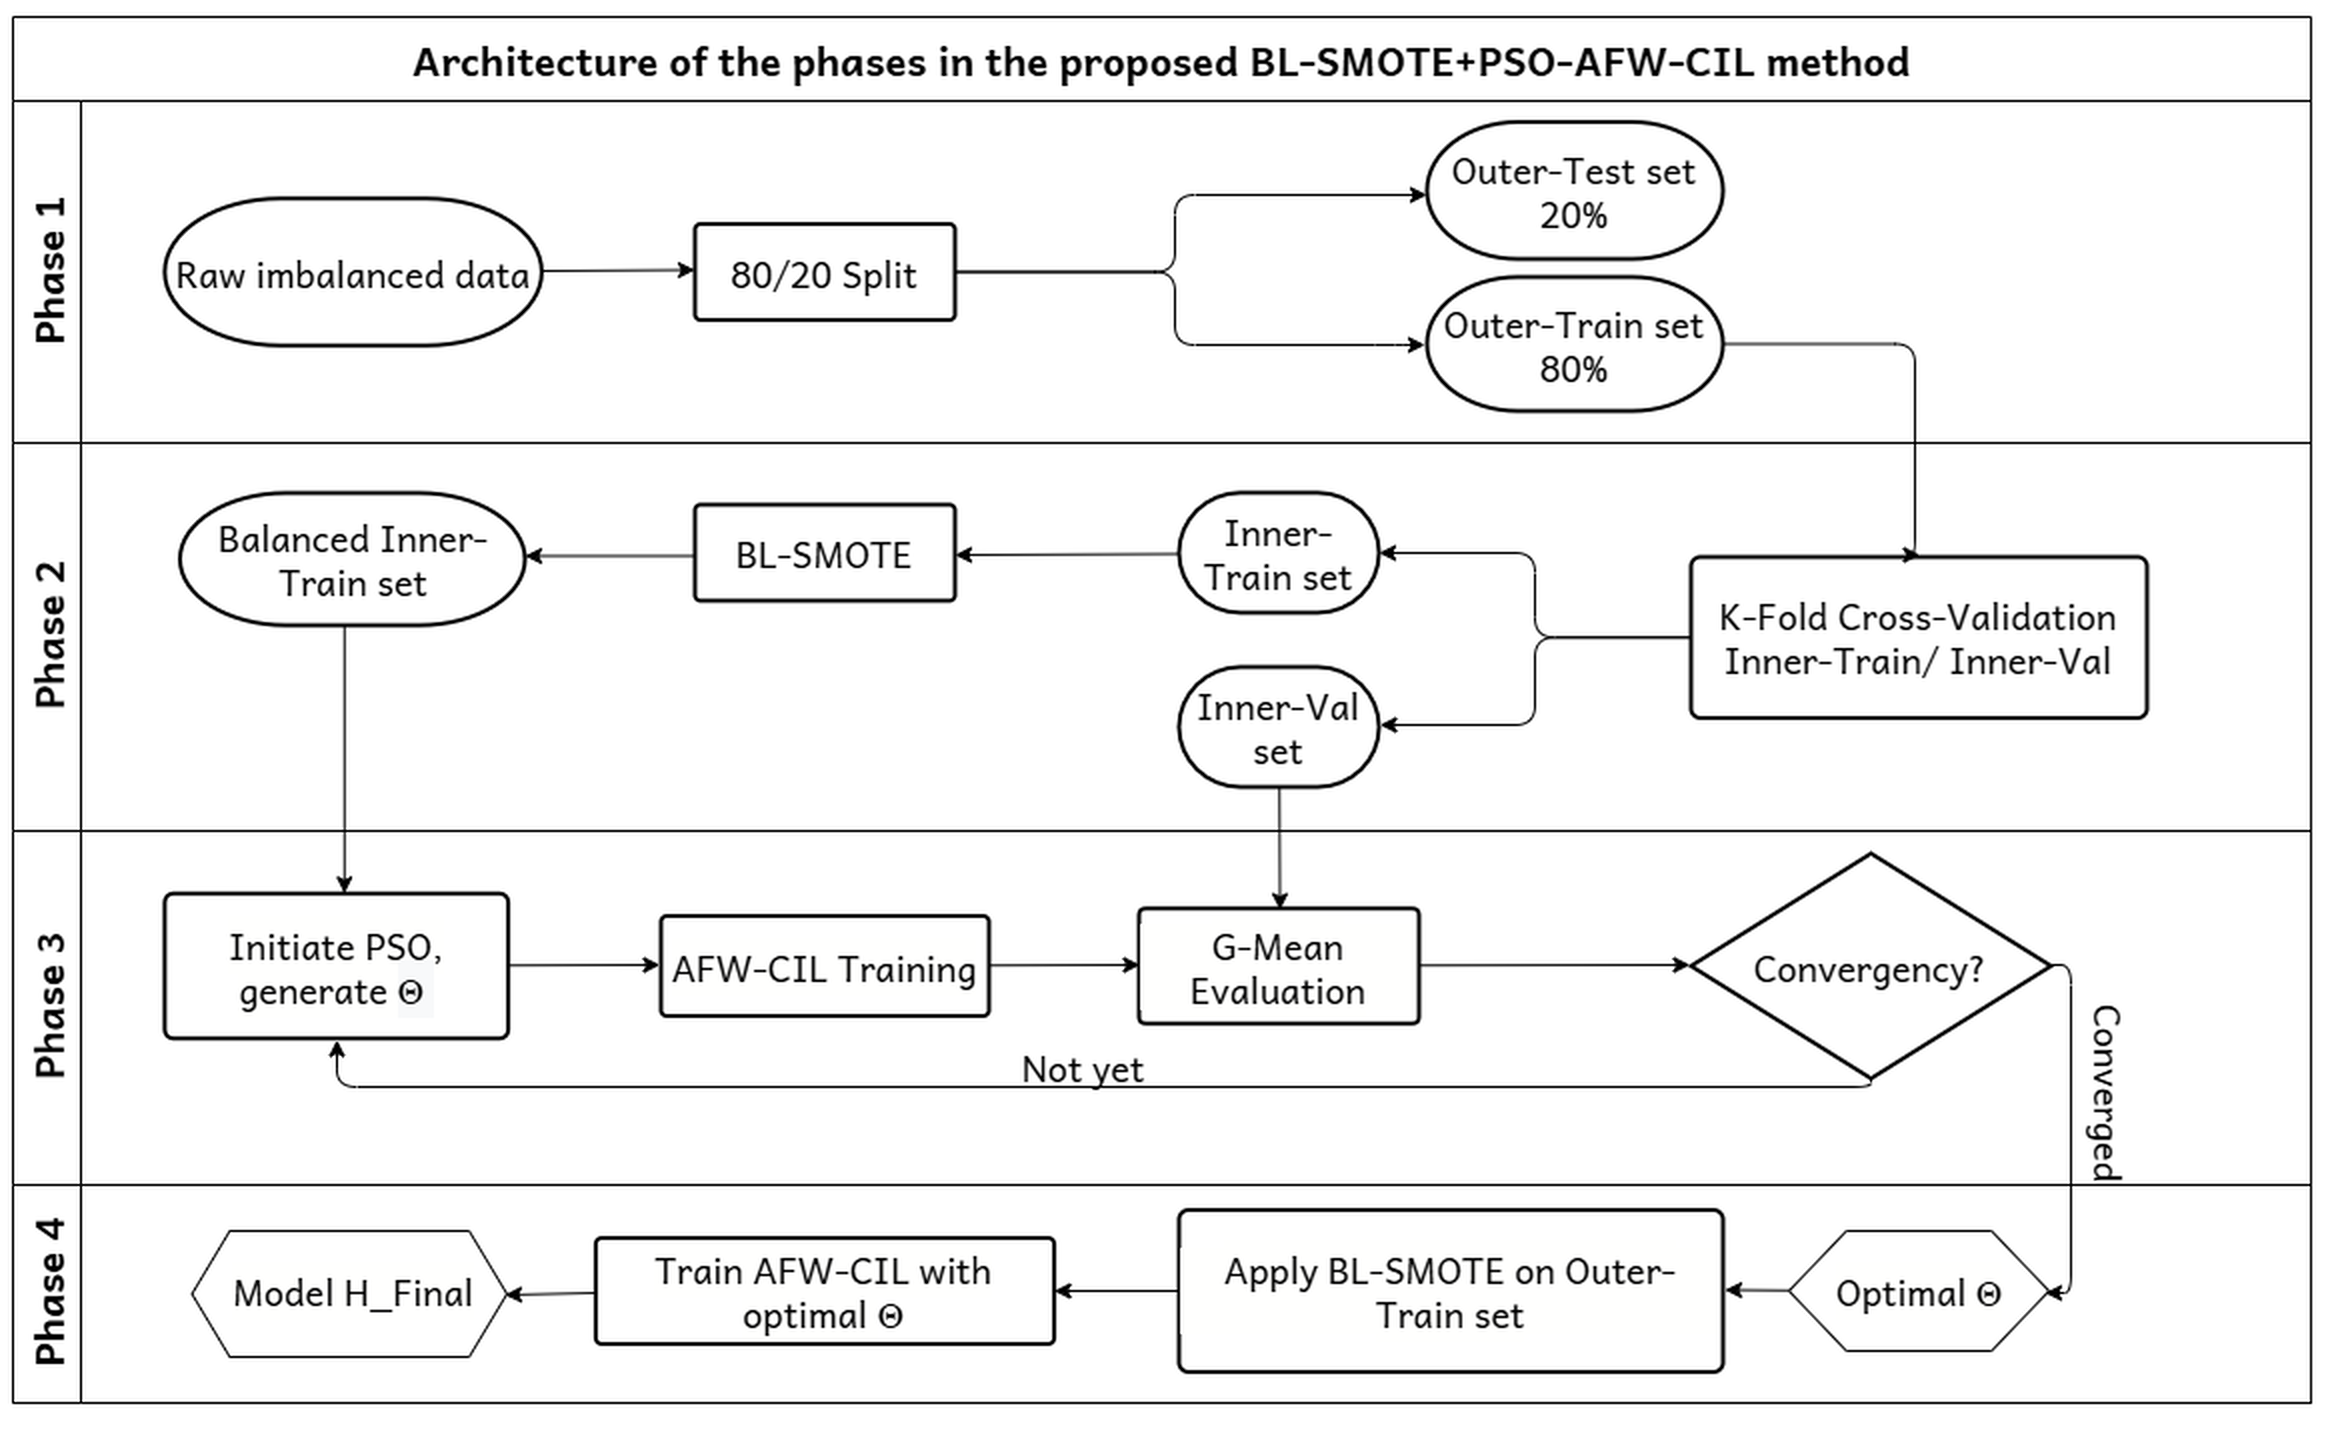
\includegraphics[width=\textwidth]{fig1(en).png}
    \caption{The four architectural phases of the proposed BL-SMOTE+PSO-AFW-CIL hybrid approach}
    \label{fig:architecture}
\end{figure*}


\subsection{Tuning AFW-CIL Hyperparameters Using PSO}\label{subsec3_1}
We employ the LDIW-PSO algorithm \cite{kennedy1995particle} to automatically tune the hyperparameters of AFW-CIL. Each particle represents a 5-dimensional position vector $\Theta = [K, \sigma_1, \sigma_2, \sigma_3, \sigma_4]$ within a search space $\Omega$. The boundaries are as follows: nearest neighbors $K \in \{3, 5, 7, 9, 11\}$; boundary shift coefficients $\sigma_1, \sigma_3 \in (0, 0.5]$; and noise penalty coefficients $\sigma_2, \sigma_4 \in (0, 1)$.

During initialization, the first particle ($i = 1$) is seeded with the default baseline coordinates $\Theta_1 = [5, 0.1, 0.5, 0.1, 0.5]$ to ensure the baseline robustness~\cite{quang2023adaptive}. The remaining $N_p-1$ particles are randomly distributed within $\Omega$.

The PSO evolution maximizes the objective function $J(\Theta)$, defined as the average $Gmean$ score across $L$ validation folds (Inner-CV):
\begin{equation} \label{eq:fitness_func}
    J(\Theta_i^t) = \frac{1}{L} \sum_{l=1}^{L} Gmean_l(\Theta_i^t) = \frac{1}{L} \sum_{l=1}^{L} \sqrt{SE_l(\Theta_i^t) \times SP_l(\Theta_i^t)} \,,
\end{equation}
where $SE_l(\Theta_i^t)$ and $SP_l(\Theta_i^t)$ denote the Sensitivity and Specificity on the $l$-th validation fold after training the AFW-CIL core on the BL-SMOTE balanced Inner-Train set using hyperparameters $\Theta_i^t$.

\smallskip
Algorithm~\ref{alg:pso} details the PSO method to tune the hyperparameters of AFW-CIL. It initializes the parameters for each particle (lines $1-5$) and performs $M$ iterations to update the velocities, positions, and fitness scores (lines $6-13$). Finally, it returns the global optimal hyperparameters $\Theta^*$.

\begin{algorithm}[H]
\small
\caption{PSO Algorithm for AFW-CIL Hyperparameter Tuning}
\label{alg:pso}
\KwIn{$\mathcal{D}_{train}$: Training dataset; $N_p$: Number of particles; $M$: Maximum iterations; $\Omega$: Search space}
\KwOut{$\Theta^*$: Global optimal hyperparameters}
\ForEach{particle $i \in \{1, 2, \dots, N_p\}$}{
    Initialize position $\Theta_i \in \Omega$ and velocity $V_i \leftarrow \mathbf{0}$\;
    $fit_i \leftarrow J(\Theta_i)$\;
    $Pbest_i \leftarrow \Theta_i$; $Pbest\_val_i \leftarrow fit_i$\;
}
$Gbest\_val \leftarrow \max_{i}(fit_i)$; $Gbest \leftarrow \Theta_i$\;
\For{$t = 1$ \KwTo $M$}{
    Update inertia weight $\omega_t$ using Eq. (\ref{eq:ldiw})\;
    \ForEach{particle $i \in \{1, 2, \dots, N_p\}$}{
        Update $V_i$ and $\Theta_i$ using Eqs. (\ref{eq:pso_v}) and (\ref{eq:pso_x})\;
        Bound coordinates of $\Theta_i$ within $\Omega$\;
        $fit_i \leftarrow J(\Theta_i)$\;
        \lIf{$fit_i > Pbest\_val_i$}{$Pbest\_val_i \leftarrow fit_i$; $Pbest_i \leftarrow \Theta_i$}
        \lIf{$fit_i > Gbest\_val$}{$Gbest\_val \leftarrow fit_i$; $Gbest \leftarrow \Theta_i$}
    }
}
\Return{$\Theta^* \leftarrow Gbest$}\;
\end{algorithm}


\subsection{The Hybrid PSO-SMOTE Approach}\label{subsec3_2}
Using the optimal hyperparameters $\Theta^* = [K, \sigma_1, \sigma_2, \sigma_3, \sigma_4]$ from the PSO module, the AFW-CIL core adjusts the fuzzy weights of sensitive samples. In this approach, the Tomek Links (TLPs) method evaluates a sample pool containing both the original training data and the synthetic borderline samples generated by BL-SMOTE.

Following the four adjustment cases in Section~\ref{subsec2_1}, the algorithm applies the PSO-tuned parameters to determine the weight adjustment. Specifically, the boundary shift coefficients ($\sigma_1$ and $\sigma_3$) control the margin adjustments for positive and negative borderline samples. Meanwhile, the noise penalty coefficients ($\sigma_2$ and $\sigma_4$) define the weight reduction for the noise samples. This allows the model to adapt to the noise and borderline characteristics of the augmented dataset without manual configuration.

\smallskip
Algorithm~\ref{alg:hybrid_approach} summarizes the execution of the proposed approach. The workflow includes splitting and normalizing data (lines~$1-2$), tuning hyperparameters via PSO (line 3), balancing training data using BL-SMOTE (line 4), and training and evaluating the final model (lines $5-6$).

\begin{algorithm}[H]
	\small
\caption{Proposed Hybrid Approach: BL-SMOTE+PSO-AFW-CIL}
\label{alg:hybrid_approach}
\KwIn{$\mathcal{D}$: Raw imbalanced dataset; $\Omega$: Parameter search space}
\KwOut{$\mathcal{H}_{final}$: Final optimal classification model; $\mathcal{M}$: Performance metrics report}
Randomly split $\mathcal{D}$ into a Training set $\mathcal{D}_{train}$ (80\%) and a Test set $\mathcal{D}_{test}$ (20\%)\;
Apply Z-score standardization to both $\mathcal{D}_{train}$ and $\mathcal{D}_{test}$\;
$\Theta^* \leftarrow$ Tune hyperparameters using Alg. \ref{alg:pso} (PSO) with inputs $(\mathcal{D}_{train}, \Omega)$\; 
$\mathcal{D}_{bal\_train} \leftarrow$ Balance training data using Alg. \ref{alg:bl_smote} (BL-SMOTE) with input $(\mathcal{D}_{train})$\;
$\mathcal{H}_{final} \leftarrow$ Train the AFW-CIL core on $\mathcal{D}_{bal\_train}$ using the optimal $\Theta^*$\;
$\mathcal{M} \leftarrow$ Evaluate $\mathcal{H}_{final}$ on $\mathcal{D}_{test}$ to calculate $SE, SP, Gmean,$ and $AUC$\;
\Return{$\mathcal{H}_{final}, \mathcal{M}$}\;
\end{algorithm}

\section{Experiments}\label{sec4}
This section evaluates the performance of the proposed hybrid PSO-SMOTE approach against baseline algorithms.

\subsection{Experimental Setup}\label{subsec4_1}
\noindent \textbf{Experimental Datasets:} We use 5 datasets from the UCI repository \cite{dua2017uci}: \textit{abalone}, \textit{haberman}, \textit{vehicle1}, \textit{transfusion}, and \textit{bankrupt}. As detailed in Table~\ref{tab:datasets}, these datasets vary in sample sizes (from 214 to 6819 samples) and feature dimensions. The class imbalance ratios also differ significantly, with the minority class proportions ranging from $35.5\%$ down to only $3.2\%$.

\begin{table}[htbp]
\caption{Detailed description of the experimental datasets from the UCI repository}\label{tab:datasets}
\begin{tabular*}{\textwidth}{@{\extracolsep\fill}llccc@{\extracolsep\fill}}
\toprule
Dataset Name & Domain  & Total samples & samples (+)/(-) &  IR (\% Pos.) \\
\midrule
abalone & Marine Biology & 4177 & 1447/2730 & 34.64 \\
haberman & Medical & 306 & 81/225 & 26.47 \\
vehicle1 & Computer Vision & 846 & 217/629 & 25.65 \\
transfusion & Medical & 748 & 178/570 & 23.80 \\
bankrupt$^1$ & Finance & 6819 & 220/6599 & 3.23 \\
\bottomrule
\end{tabular*}
\smallskip
\noindent \footnotesize \textbf{Source:} Extracted from the UCI Machine Learning Repository. \\
\noindent \footnotesize $^1$Full name: Company Bankruptcy Prediction.
\end{table}

\smallskip
\noindent \textbf{Evaluation Strategy \& Scenarios:} To evaluate the model effectiveness, we design three experimental scenarios for the 5 selected datasets. The first experiment is to evaluate the hyperparameter tuning capability of the PSO algorithm on the original data. The second experiment is to compare the classification performance of the proposed hybrid method against the baselines. The last experiment is to test the model's predictive stability under gradually decreasing minority class ratios (down to $\le 2\%$). 

\smallskip
\noindent \textbf{Metrics \& Parameters:} Performance is evaluated using Sensitivity ($SE$), Specificity ($SP$), Geometric Mean ($Gmean$), F1-score, and $AUC$ (focusing on $SE$, $Gmean$, and $AUC$) via repeated 5-fold cross-validation (Mean $\pm$ Std). Parameters are configured as follows: \textbf{W-SVM}: Linear kernel, $C=100$; \textbf{PSO}: Swarm size $N_p=5$, iterations $M=5$, $\omega \in [0.9, 0.4]$, TVAC $c_1 \in [2.5, 0.5]$ and $c_2 \in [0.5, 2.5]$; \textbf{AFW-CIL\_default}: $K=5$, $\sigma_{1,3}=0.1$, $\sigma_{2,4}=0.5$; \textbf{BL-SMOTE}: $K=5$.


\subsection{Experimental Results}\label{subsec4_2}
\smallskip
\noindent \textbf{Experiment 1 (PSO Evaluation):} Table~\ref{tab:results_scenario1} details the classification performance of the tuning methods on the raw imbalanced datasets.

\begin{table*}[htbp]
\caption{Performance comparison of tuning methods on the 5 representative benchmark datasets (Mean $\pm$ Std)}\label{tab:results_scenario1}
\resizebox{\textwidth}{!}{%
\begin{tabular}{llccccc}
\toprule
Dataset & Method & SE & SP & Gmean & F1-Score & AUC \\
\midrule
% --- Dữ liệu 1: GLASS ---

% --- Dữ liệu 2: ABALONE ---
\multirow{4}{*}{\textbf{\textit{abalone}}}
& W-SVM & $0.648 \pm 0.026$ & $\mathbf{0.855 \pm 0.011}$ & $\mathbf{0.744 \pm 0.017}$ & $\mathbf{0.674 \pm 0.021}$ & $\mathbf{0.751 \pm 0.015}$ \\
& AFW-CIL$_{\mathrm{default}}$ & $0.654 \pm 0.025$ & $0.841 \pm 0.017$ & $0.741 \pm 0.014$ & $0.669 \pm 0.018$ & $0.747 \pm 0.013$ \\
& GridSearch-AFW & $0.654 \pm 0.027$ & $0.838 \pm 0.020$ & $0.740 \pm 0.014$ & $0.667 \pm 0.018$ & $0.746 \pm 0.013$ \\
& PSO-AFW-CIL & $\mathbf{0.661 \pm 0.044}$ & $0.832 \pm 0.025$ & $0.741 \pm 0.019$ & $0.668 \pm 0.023$ & $0.746 \pm 0.017$ \\
\midrule
% --- Dữ liệu 2: haberman ---
\multirow{4}{*}{\textbf{\textit{haberman}}}
& W-SVM & $0.202 \pm 0.165$ & $\mathbf{0.921 \pm 0.071}$ & $0.334 \pm 0.258$ & $0.242 \pm 0.193$ & $0.561 \pm 0.057$ \\
& AFW-CIL$_{\mathrm{default}}$ & $\mathbf{0.375 \pm 0.110}$ & $0.865 \pm 0.044$ & $\mathbf{0.563 \pm 0.086}$ & $\mathbf{0.424 \pm 0.102}$ & $\mathbf{0.620 \pm 0.059}$ \\
& GridSearch-AFW & $0.372 \pm 0.107$ & $0.866 \pm 0.052$ & $0.562 \pm 0.084$ & $0.424 \pm 0.101$ & $0.619 \pm 0.059$ \\
& PSO-AFW-CIL & $0.307 \pm 0.185$ & $0.881 \pm 0.075$ & $0.452 \pm 0.242$ & $0.339 \pm 0.196$ & $0.594 \pm 0.073$ \\
\midrule
% --- Dữ liệu 3: VEHICLE1  ---
\multirow{4}{*}{\textbf{\textit{vehicle1}}}
& W-SVM & $0.626 \pm 0.057$ & $\mathbf{0.867 \pm 0.024}$ & $0.736 \pm 0.032$ & $0.622 \pm 0.038$ & $0.747 \pm 0.027$ \\
& AFW-CIL$_{\mathrm{default}}$ & $0.642 \pm 0.061$ & $0.854 \pm 0.024$ & $0.740 \pm 0.035$ & $0.622 \pm 0.044$ & $0.748 \pm 0.031$ \\
& GridSearch-AFW & $0.644 \pm 0.059$ & $0.855 \pm 0.021$ & $0.741 \pm 0.035$ & $0.623 \pm 0.043$ & $0.750 \pm 0.031$ \\
& PSO-AFW-CIL & $\mathbf{0.663 \pm 0.062}$ & $0.848 \pm 0.030$ & $\mathbf{0.749 \pm 0.035}$ & $\mathbf{0.630 \pm 0.043}$ & $\mathbf{0.756 \pm 0.031}$ \\
\midrule
% --- Dữ liệu 4: Transfusion  ---
\multirow{4}{*}{\textbf{\textit{transfusion}}}
& W-SVM & $0.087 \pm 0.135$ & $\mathbf{0.967 \pm 0.052}$ & $0.157 \pm 0.234$ & $0.108 \pm 0.165$ & $0.527 \pm 0.045$ \\
& AFW-CIL$_{\mathrm{default}}$ & $\mathbf{0.582 \pm 0.081}$ & $0.758 \pm 0.045$ & $\mathbf{0.662 \pm 0.043}$ & $\mathbf{0.493 \pm 0.049}$ & $\mathbf{0.670 \pm 0.038}$ \\
& GridSearch-AFW & $0.531 \pm 0.087$ & $0.799 \pm 0.057$ & $0.648 \pm 0.051$ & $0.488 \pm 0.057$ & $0.665 \pm 0.039$ \\
& PSO-AFW-CIL & $0.545 \pm 0.095$ & $0.789 \pm 0.050$ & $0.652 \pm 0.052$ & $0.489 \pm 0.058$ & $0.667 \pm 0.041$ \\
\midrule
% --- Dữ liệu 5: Bankrupt  ---
\multirow{4}{*}{\textbf{\textit{bankrupt}}}
& W-SVM & $0.195 \pm 0.044$ & $\mathbf{0.990 \pm 0.003}$ & $0.437 \pm 0.051$ & $0.259 \pm 0.053$ & $0.593 \pm 0.022$ \\
& AFW-CIL$_{\mathrm{default}}$ & $\mathbf{0.545 \pm 0.062}$ & $0.956 \pm 0.007$ & $\mathbf{0.721 \pm 0.038}$ & $0.380 \pm 0.013$ & $\mathbf{0.751 \pm 0.028}$ \\
& GridSearch-AFW & $0.541 \pm 0.049$ & $0.956 \pm 0.005$ & $0.718 \pm 0.031$ & $0.376 \pm 0.018$ & $0.748 \pm 0.023$ \\
& PSO-AFW-CIL & $0.536 \pm 0.061$ & $0.957 \pm 0.007$ & $0.716 \pm 0.039$ & $\mathbf{0.381 \pm 0.017}$ & $0.747 \pm 0.028$ \\
\bottomrule
\end{tabular}
}

\smallskip
\noindent \footnotesize \textbf{Note:} Bold values indicate the highest average results for each dataset. Several method names are abbreviated (e.g., \textit{GridSearch-AFW} instead of \textit{GridSearch-AFW-CIL}) to save space.
\end{table*}

\smallskip
Table~\ref{tab:results_scenario1} shows that the AFW-CIL variants consistently improve performance over the W-SVM baseline. By automating hyperparameter tuning, PSO-AFW-CIL achieves comparable or higher $SE$ and $Gmean$ scores than the manual setup and GridSearch. This integration eliminates manual trial-and-error without sacrificing classification accuracy.


\smallskip
\noindent \textbf{Experiment 2 (Hybrid Approach):} Table~\ref{tab:results_scenario2} summarizes the classification performance of the proposed hybrid approach against the baseline algorithms.

\begin{table*}[htbp]
\caption{Performance comparison of the hybrid approach on the 5 representative benchmark datasets (Mean $\pm$ Std)}\label{tab:results_scenario2}
\resizebox{\textwidth}{!}{%
\begin{tabular}{llccccc}
\toprule
Dataset & Method & SE & SP & Gmean & F1-Score & AUC \\
\midrule
% --- Dữ liệu 2: VEHICLE1 ---
\multirow{4}{*}{\textbf{\textit{vehicle1}}}
& W-SVM & $0.626 \pm 0.057$ & $\mathbf{0.867 \pm 0.024}$ & $0.736 \pm 0.032$ & $0.622 \pm 0.038$ & $0.747 \pm 0.027$ \\
& AFW-CIL$_{\mathrm{default}}$ & $0.642 \pm 0.061$ & $0.854 \pm 0.024$ & $0.740 \pm 0.035$ & $0.622 \pm 0.044$ & $0.748 \pm 0.031$ \\
& PSO-AFW-CIL & $0.655 \pm 0.058$ & $0.850 \pm 0.028$ & $0.746 \pm 0.033$ & $0.627 \pm 0.041$ & $0.753 \pm 0.030$ \\
& BL-SMOTE+PSO-AFW & $\mathbf{0.787 \pm 0.050}$ & $0.799 \pm 0.026$ & $\mathbf{0.792 \pm 0.024}$ & $\mathbf{0.664 \pm 0.030}$ & $\mathbf{0.793 \pm 0.024}$ \\
\midrule
% --- Dữ liệu 2: HABERMAN ---
\multirow{4}{*}{\textbf{\textit{haberman}}} 
& W-SVM &  $0.202 \pm 0.165$  &  $\mathbf{0.921 \pm 0.071}$  &  $0.334 \pm 0.258$  &  $0.242 \pm 0.193$  &  $0.561 \pm 0.057$  \\
& AFW-CIL $_{\mathrm{default}}$   &  $0.375 \pm 0.110$  &  $0.865 \pm 0.044$  &  $0.563 \pm 0.086$  &  $0.424 \pm 0.102$  &  $\mathbf{0.620 \pm 0.059}$  \\
& PSO-AFW-CIL       &  $0.275 \pm 0.204$  &  $0.888 \pm 0.084$  &  $0.397 \pm 0.273$  &  $0.297 \pm 0.215$  &  $0.582 \pm 0.075$  \\
& BL-SMOTE+PSO-AFW  &  $\mathbf{0.577 \pm 0.157}$  &  $0.635 \pm 0.170$  &  $\mathbf{0.575 \pm 0.142}$  &  $\mathbf{0.446 \pm 0.088}$  &  $0.606 \pm 0.072$  \\
\midrule
% --- Dữ liệu 3: TRANSFUSION ---
\multirow{4}{*}{\textbf{\textit{transfusion}}}
& W-SVM & $0.087 \pm 0.135$ & $\mathbf{0.967 \pm 0.052}$ & $0.157 \pm 0.234$ & $0.108 \pm 0.165$ & $0.527 \pm 0.045$ \\
& AFW-CIL$_{\mathrm{default}}$ & $0.582 \pm 0.081$ & $0.758 \pm 0.045$ & $0.662 \pm 0.043$ & $0.493 \pm 0.049$ & $0.670 \pm 0.038$ \\
& PSO-AFW-CIL & $0.530 \pm 0.111$ & $0.790 \pm 0.059$ & $0.641 \pm 0.063$ & $0.477 \pm 0.064$ & $0.660 \pm 0.040$ \\
& BL-SMOTE+PSO-AFW & $\mathbf{0.759 \pm 0.070}$ & $0.613 \pm 0.055$ & $\mathbf{0.680 \pm 0.039}$ & $\mathbf{0.506 \pm 0.041}$ & $\mathbf{0.686 \pm 0.039}$ \\
\midrule
% --- Dữ liệu 4: ABALONE ---
\multirow{4}{*}{\textbf{\textit{abalone}}}
& W-SVM & $0.648 \pm 0.026$ & $\mathbf{0.855 \pm 0.011}$ & $0.744 \pm 0.017$ & $0.674 \pm 0.021$ & $0.751 \pm 0.015$ \\
& AFW-CIL$_{\mathrm{default}}$ & $0.654 \pm 0.025$ & $0.841 \pm 0.017$ & $0.741 \pm 0.014$ & $0.669 \pm 0.018$ & $0.747 \pm 0.013$ \\
& PSO-AFW-CIL & $0.667 \pm 0.025$ & $0.827 \pm 0.022$ & $0.743 \pm 0.013$ & $0.669 \pm 0.017$ & $0.747 \pm 0.013$ \\
& BL-SMOTE+PSO-AFW & $\mathbf{0.786 \pm 0.036}$ & $0.746 \pm 0.015$ & $\mathbf{0.765 \pm 0.020}$ & $\mathbf{0.694 \pm 0.024}$ & $\mathbf{0.766 \pm 0.021}$ \\
\midrule
% --- Dữ liệu 5: BANKRUPT ---
\multirow{4}{*}{\textbf{\textit{bankrupt}}}
& W-SVM & $0.195 \pm 0.044$ & $\mathbf{0.990 \pm 0.003}$ & $0.437 \pm 0.051$ & $0.259 \pm 0.053$ & $0.593 \pm 0.022$ \\
& AFW-CIL$_{\mathrm{default}}$ & $0.545 \pm 0.062$ & $0.956 \pm 0.007$ & $0.721 \pm 0.038$ & $0.380 \pm 0.013$ & $0.751 \pm 0.028$ \\
& PSO-AFW-CIL & $0.545 \pm 0.051$ & $0.956 \pm 0.007$ & $0.722 \pm 0.031$ & $\mathbf{0.382 \pm 0.007}$ & $0.751 \pm 0.022$ \\
& BL-SMOTE+PSO-AFW & $\mathbf{0.609 \pm 0.037}$ & $0.931 \pm 0.006$ & $\mathbf{0.753 \pm 0.022}$ & $0.332 \pm 0.016$ & $\mathbf{0.770 \pm 0.017}$ \\
\bottomrule
\end{tabular}
}

\smallskip
\noindent \footnotesize \textbf{Note:} Bold values indicate the highest average results for each dataset. Several method names are abbreviated (e.g., \textit{BL-SMOTE+PSO-AFW} instead of \textit{BL-SMOTE+PSO-AFW-CIL}) to save space.
\end{table*}

\smallskip
Table~\ref{tab:results_scenario2} shows that the baseline algorithms yield low Sensitivity ($SE$) due to data sparsity. In contrast, the BL-SMOTE+PSO-AFW-CIL approach improves both $SE$ and $Gmean$. The PSO-tuned AFW-CIL core acts as an adaptive noise filter to integrate synthetic borderline samples without degrading Specificity ($SP$). This combination of data-level enrichment and algorithm-level tuning improves overall classification performance.


\smallskip 
\noindent \textbf{Experiment 3 (Stress-test):} Table~\ref{tab:scenario3} and Figures~\ref{fig:scenario3_se}--\ref{fig:scenario3_auc} detail the robustness of the models under data scarcity with decreasing minority class ratios.
\begin{table*}[htbp]
\caption{Performance evaluation under decreasing minority class ratios (Mean $\pm$ Std)}\label{tab:scenario3}
\resizebox{\textwidth}{!}{%
\begin{tabular}{lllcccccc}
\toprule
Dataset & IR (\%) & Method & SE & SP & Gmean & F1-Score & Accuracy & AUC \\
\midrule
% --- abalone ---
\multirow{12}{*}{\textbf{\textit{abalone}}} 
& \multirow{3}{*}{8}
& W-SVM     & $0.000 \pm 0.000$ & $\mathbf{1.000 \pm 0.000}$ & $0.000 \pm 0.000$ & $0.000 \pm 0.000$ & $\mathbf{0.920 \pm 0.001}$ & $0.500 \pm 0.000$ \\
& & AFW     & $0.451 \pm 0.066$ & $0.929 \pm 0.008$ & $0.646 \pm 0.045$ & $\mathbf{0.397 \pm 0.041}$ & $0.891 \pm 0.007$ & $0.690 \pm 0.031$ \\
& & Proposed& $\mathbf{0.717 \pm 0.086}$ & $0.819 \pm 0.018$ & $\mathbf{0.765 \pm 0.048}$ & $0.378 \pm 0.045$ & $0.811 \pm 0.019$ & $\mathbf{0.768 \pm 0.045}$ \\
\cmidrule{2-9}
& \multirow{3}{*}{6}
& W-SVM     & $0.000 \pm 0.000$ & $\mathbf{1.000 \pm 0.000}$ & $0.000 \pm 0.000$ & $0.000 \pm 0.000$ & $\mathbf{0.940 \pm 0.001}$ & $0.500 \pm 0.000$ \\
& & AFW     & $0.391 \pm 0.062$ & $0.928 \pm 0.014$ & $0.601 \pm 0.052$ & $\mathbf{0.313 \pm 0.059}$ & $0.896 \pm 0.016$ & $0.660 \pm 0.035$ \\
& & Proposed& $\mathbf{0.656 \pm 0.124}$ & $0.794 \pm 0.036$ & $\mathbf{0.718 \pm 0.053}$ & $0.267 \pm 0.019$ & $0.786 \pm 0.027$ & $\mathbf{0.725 \pm 0.047}$ \\
\cmidrule{2-9}
& \multirow{3}{*}{4}
& W-SVM     & $0.000 \pm 0.000$ & $\mathbf{1.000 \pm 0.000}$ & $0.000 \pm 0.000$ & $0.000 \pm 0.000$ & $\mathbf{0.960 \pm 0.001}$ & $0.500 \pm 0.000$ \\
& & AFW     & $0.400 \pm 0.132$ & $0.943 \pm 0.011$ & $0.607 \pm 0.104$ & $\mathbf{0.285 \pm 0.083}$ & $0.921 \pm 0.011$ & $0.671 \pm 0.066$ \\
& & Proposed& $\mathbf{0.585 \pm 0.098}$ & $0.866 \pm 0.011$ & $\mathbf{0.710 \pm 0.058}$ & $0.242 \pm 0.034$ & $0.855 \pm 0.010$ & $\mathbf{0.725 \pm 0.047}$ \\
\cmidrule{2-9}
& \multirow{3}{*}{2}
& W-SVM     & $0.000 \pm 0.000$ & $\mathbf{1.000 \pm 0.000}$ & $0.000 \pm 0.000$ & $0.000 \pm 0.000$ & $\mathbf{0.980 \pm 0.000}$ & $0.500 \pm 0.000$ \\
& & AFW     & $0.309 \pm 0.228$ & $0.948 \pm 0.011$ & $0.475 \pm 0.286$ & $\mathbf{0.149 \pm 0.093}$ & $0.936 \pm 0.008$ & $0.629 \pm 0.110$ \\
& & Proposed& $\mathbf{0.618 \pm 0.119}$ & $0.859 \pm 0.026$ & $\mathbf{0.725 \pm 0.059}$ & $0.144 \pm 0.020$ & $0.854 \pm 0.024$ & $\mathbf{0.738 \pm 0.051}$ \\
\midrule
% --- 1. haberman ---
\multirow{12}{*}{\textbf{\textit{haberman}}} 
& \multirow{3}{*}{8}
& W-SVM     & $0.000 \pm 0.000$ & $\mathbf{1.000 \pm 0.000}$ & $0.000 \pm 0.000$ & $0.000 \pm 0.000$ & $\mathbf{0.922 \pm 0.008}$ & $0.500 \pm 0.000$ \\
& & AFW     & $0.337 \pm 0.258$ & $0.932 \pm 0.037$ & $0.469 \pm 0.302$ & $0.282 \pm 0.199$ & $0.885 \pm 0.031$ & $0.634 \pm 0.122$ \\
& & Proposed& $\mathbf{0.543 \pm 0.220}$ & $0.820 \pm 0.075$ & $\mathbf{0.643 \pm 0.180}$ & $\mathbf{0.304 \pm 0.127}$ & $0.799 \pm 0.071$ & $\mathbf{0.682 \pm 0.116}$ \\
\cmidrule{2-9}
& \multirow{3}{*}{6}
& W-SVM     & $0.000 \pm 0.000$ & $\mathbf{1.000 \pm 0.000}$ & $0.000 \pm 0.000$ & $0.000 \pm 0.000$ & $\mathbf{0.941 \pm 0.008}$ & $0.500 \pm 0.000$ \\
& & AFW     & $0.087 \pm 0.172$ & $0.915 \pm 0.048$ & $0.130 \pm 0.250$ & $0.058 \pm 0.113$ & $0.866 \pm 0.043$ & $0.501 \pm 0.086$ \\
& & Proposed& $\mathbf{0.360 \pm 0.288}$ & $0.816 \pm 0.068$ & $\mathbf{0.448 \pm 0.299}$ & $\mathbf{0.165 \pm 0.126}$ & $0.790 \pm 0.061$ & $\mathbf{0.588 \pm 0.139}$ \\
\cmidrule{2-9}
& \multirow{3}{*}{4}
& W-SVM     & $0.000 \pm 0.000$ & $\mathbf{1.000 \pm 0.000}$ & $0.000 \pm 0.000$ & $0.000 \pm 0.000$ & $\mathbf{0.962 \pm 0.008}$ & $0.500 \pm 0.000$ \\
& & AFW     & $0.200 \pm 0.286$ & $0.924 \pm 0.046$ & $0.256 \pm 0.348$ & $\mathbf{0.136 \pm 0.205}$ & $0.896 \pm 0.043$ & $0.562 \pm 0.143$ \\
& & Proposed& $\mathbf{0.290 \pm 0.336}$ & $0.854 \pm 0.064$ & $\mathbf{0.337 \pm 0.362}$ & $0.120 \pm 0.154$ & $0.833 \pm 0.059$ & $\mathbf{0.572 \pm 0.162}$ \\
\cmidrule{2-9}
& \multirow{3}{*}{2}
& W-SVM     & $\mathbf{0.000 \pm 0.000}$ & $\mathbf{1.000 \pm 0.000}$ & $\mathbf{0.000 \pm 0.000}$ & $\mathbf{0.000 \pm 0.000}$ & $\mathbf{0.983 \pm 0.000}$ & $\mathbf{0.500 \pm 0.000}$ \\
& & AFW     & $\mathbf{0.000 \pm 0.000}$ & $0.939 \pm 0.056$ & $\mathbf{0.000 \pm 0.000}$ & $\mathbf{0.000 \pm 0.000}$ & $0.923 \pm 0.055$ & $0.470 \pm 0.028$ \\
& & Proposed& $\mathbf{0.000 \pm 0.000}$ & $0.588 \pm 0.463$ & $\mathbf{0.000 \pm 0.000}$ & $\mathbf{0.000 \pm 0.000}$ & $0.577 \pm 0.455$ & $0.470 \pm 0.025$ \\
\midrule
% --- vehicle1 ---
\multirow{12}{*}{\textbf{\textit{vehicle1}}} 
& \multirow{3}{*}{8}
& W-SVM     & $0.405 \pm 0.168$ & $\mathbf{0.964 \pm 0.017}$ & $0.601 \pm 0.172$ & $\mathbf{0.430 \pm 0.156}$ & $\mathbf{0.920 \pm 0.016}$ & $0.685 \pm 0.082$ \\
& & AFW     & $0.477 \pm 0.180$ & $0.913 \pm 0.027$ & $0.647 \pm 0.124$ & $0.376 \pm 0.105$ & $0.878 \pm 0.023$ & $0.695 \pm 0.085$ \\
& & Proposed& $\mathbf{0.568 \pm 0.170}$ & $0.858 \pm 0.027$ & $\mathbf{0.689 \pm 0.106}$ & $0.348 \pm 0.080$ & $0.835 \pm 0.022$ & $\mathbf{0.713 \pm 0.080}$ \\
\cmidrule{2-9}
& \multirow{3}{*}{6}
& W-SVM     & $0.000 \pm 0.000$ & $\mathbf{1.000 \pm 0.000}$ & $0.000 \pm 0.000$ & $0.000 \pm 0.000$ & $\mathbf{0.940 \pm 0.000}$ & $0.500 \pm 0.000$ \\
& & AFW     & $0.315 \pm 0.174$ & $0.929 \pm 0.017$ & $0.514 \pm 0.171$ & $0.252 \pm 0.125$ & $0.893 \pm 0.018$ & $0.622 \pm 0.086$ \\
& & Proposed& $\mathbf{0.570 \pm 0.211}$ & $0.871 \pm 0.030$ & $\mathbf{0.689 \pm 0.147}$ & $\mathbf{0.314 \pm 0.111}$ & $0.853 \pm 0.028$ & $\mathbf{0.721 \pm 0.103}$ \\
\cmidrule{2-9}
& \multirow{3}{*}{4}
& W-SVM     & $0.023 \pm 0.085$ & $\mathbf{0.993 \pm 0.013}$ & $0.041 \pm 0.144$ & $0.020 \pm 0.070$ & $\mathbf{0.955 \pm 0.011}$ & $0.508 \pm 0.038$ \\
& & AFW     & $0.367 \pm 0.208$ & $0.936 \pm 0.024$ & $0.538 \pm 0.236$ & $0.253 \pm 0.144$ & $0.913 \pm 0.025$ & $0.651 \pm 0.106$ \\
& & Proposed& $\mathbf{0.481 \pm 0.244}$ & $0.917 \pm 0.027$ & $\mathbf{0.624 \pm 0.230}$ & $\mathbf{0.270 \pm 0.127}$ & $0.899 \pm 0.027$ & $\mathbf{0.699 \pm 0.121}$ \\
\cmidrule{2-9}
& \multirow{3}{*}{2}
& W-SVM     & $0.000 \pm 0.000$ & $\mathbf{1.000 \pm 0.001}$ & $0.000 \pm 0.000$ & $0.000 \pm 0.000$ & $\mathbf{0.981 \pm 0.004}$ & $0.500 \pm 0.001$ \\
& & AFW     & $\mathbf{0.087 \pm 0.181}$ & $0.958 \pm 0.026$ & $\mathbf{0.127 \pm 0.261}$ & $\mathbf{0.041 \pm 0.089}$ & $0.942 \pm 0.025$ & $\mathbf{0.522 \pm 0.087}$ \\
& & Proposed& $0.067 \pm 0.160$ & $0.960 \pm 0.024$ & $0.100 \pm 0.235$ & $0.034 \pm 0.083$ & $0.944 \pm 0.023$ & $0.513 \pm 0.078$ \\
\midrule
% --- transfusion ---
\multirow{12}{*}{\textbf{\textit{transfusion}}} 
& \multirow{3}{*}{8}
& W-SVM     & $0.000 \pm 0.000$ & $\mathbf{1.000 \pm 0.000}$ & $0.000 \pm 0.000$ & $0.000 \pm 0.000$ & $\mathbf{0.921 \pm 0.003}$ & $0.500 \pm 0.000$ \\
& & AFW     & $0.259 \pm 0.151$ & $0.881 \pm 0.036$ & $0.443 \pm 0.172$ & $0.189 \pm 0.097$ & $0.832 \pm 0.030$ & $0.570 \pm 0.070$ \\
& & Proposed& $\mathbf{0.673 \pm 0.148}$ & $0.698 \pm 0.046$ & $\mathbf{0.681 \pm 0.073}$ & $\mathbf{0.260 \pm 0.053}$ & $0.696 \pm 0.041$ & $\mathbf{0.686 \pm 0.072}$ \\
\cmidrule{2-9}
& \multirow{3}{*}{6}
& W-SVM     & $0.000 \pm 0.000$ & $\mathbf{1.000 \pm 0.000}$ & $0.000 \pm 0.000$ & $0.000 \pm 0.000$ & $\mathbf{0.941 \pm 0.003}$ & $0.500 \pm 0.000$ \\
& & AFW     & $0.236 \pm 0.144$ & $0.943 \pm 0.035$ & $0.435 \pm 0.184$ & $\mathbf{0.222 \pm 0.134}$ & $0.901 \pm 0.034$ & $0.590 \pm 0.074$ \\
& & Proposed& $\mathbf{0.651 \pm 0.246}$ & $0.697 \pm 0.046$ & $\mathbf{0.657 \pm 0.135}$ & $0.199 \pm 0.067$ & $0.694 \pm 0.040$ & $\mathbf{0.674 \pm 0.117}$ \\
\cmidrule{2-9}
& \multirow{3}{*}{4}
& W-SVM     & $0.000 \pm 0.000$ & $\mathbf{1.000 \pm 0.000}$ & $0.000 \pm 0.000$ & $0.000 \pm 0.000$ & $\mathbf{0.961 \pm 0.004}$ & $0.500 \pm 0.000$ \\
& & AFW     & $0.150 \pm 0.176$ & $0.958 \pm 0.023$ & $0.267 \pm 0.270$ & $0.123 \pm 0.134$ & $0.926 \pm 0.021$ & $0.554 \pm 0.085$ \\
& & Proposed& $\mathbf{0.597 \pm 0.263}$ & $0.761 \pm 0.061$ & $\mathbf{0.638 \pm 0.202}$ & $\mathbf{0.155 \pm 0.070}$ & $0.755 \pm 0.053$ & $\mathbf{0.679 \pm 0.119}$ \\
\cmidrule{2-9}
& \multirow{3}{*}{2}
& W-SVM     & $0.000 \pm 0.000$ & $\mathbf{1.000 \pm 0.001}$ & $0.000 \pm 0.000$ & $0.000 \pm 0.000$ & $\mathbf{0.981 \pm 0.004}$ & $0.500 \pm 0.001$ \\
& & AFW     & $0.463 \pm 0.360$ & $0.954 \pm 0.021$ & $0.552 \pm 0.369$ & $\mathbf{0.216 \pm 0.163}$ & $0.945 \pm 0.018$ & $0.709 \pm 0.175$ \\
& & Proposed& $\mathbf{0.647 \pm 0.299}$ & $0.874 \pm 0.069$ & $\mathbf{0.712 \pm 0.224}$ & $0.164 \pm 0.077$ & $0.869 \pm 0.065$ & $\mathbf{0.760 \pm 0.137}$ \\
\midrule
% --- bankrupt ---
\multirow{12}{*}{\textbf{\textit{bankrupt}}}
& \multirow{3}{*}{3}
& W-SVM     & $0.181 \pm 0.045$ & $\mathbf{0.992 \pm 0.003}$ & $0.422 \pm 0.054$ & $0.251 \pm 0.041$ & $\mathbf{0.968 \pm 0.002}$ & $0.587 \pm 0.021$ \\
& & AFW     & $0.549 \pm 0.087$ & $0.956 \pm 0.008$ & $0.723 \pm 0.060$ & $\mathbf{0.372 \pm 0.069}$ & $0.944 \pm 0.009$ & $0.753 \pm 0.045$ \\
& & Proposed& $\mathbf{0.603 \pm 0.054}$ & $0.931 \pm 0.006$ & $\mathbf{0.749 \pm 0.034}$ & $0.316 \pm 0.027$ & $0.922 \pm 0.006$ & $\mathbf{0.767 \pm 0.027}$ \\
\cmidrule{2-9}
& \multirow{3}{*}{2}
& W-SVM     & $0.097 \pm 0.043$ & $\mathbf{0.995 \pm 0.003}$ & $0.304 \pm 0.074$ & $0.148 \pm 0.068$ & $\mathbf{0.978 \pm 0.003}$ & $0.546 \pm 0.022$ \\
& & AFW     & $0.486 \pm 0.079$ & $0.958 \pm 0.007$ & $0.681 \pm 0.054$ & $0.277 \pm 0.042$ & $0.949 \pm 0.007$ & $0.722 \pm 0.039$ \\
& & Proposed& $\mathbf{0.569 \pm 0.147}$ & $0.950 \pm 0.013$ & $\mathbf{0.730 \pm 0.092}$ & $\mathbf{0.281 \pm 0.053}$ & $0.942 \pm 0.012$ & $\mathbf{0.759 \pm 0.070}$ \\
\cmidrule{2-9}
& \multirow{3}{*}{1}
& W-SVM     & $0.045 \pm 0.068$ & $\mathbf{0.997 \pm 0.003}$ & $0.132 \pm 0.185$ & $0.054 \pm 0.076$ & $\mathbf{0.987 \pm 0.002}$ & $0.521 \pm 0.033$ \\
& & AFW     & $\mathbf{0.349 \pm 0.170}$ & $0.973 \pm 0.001$ & $\mathbf{0.569 \pm 0.141}$ & $\mathbf{0.171 \pm 0.076}$ & $0.967 \pm 0.002$ & $\mathbf{0.661 \pm 0.085}$ \\
& & Proposed& $0.347 \pm 0.218$ & $0.966 \pm 0.006$ & $0.558 \pm 0.173$ & $0.146 \pm 0.086$ & $0.960 \pm 0.006$ & $0.657 \pm 0.109$ \\
\cmidrule{2-9}
& \multirow{3}{*}{0.5}
& W-SVM     & $0.091 \pm 0.083$ & $\mathbf{0.995 \pm 0.002}$ & $0.232 \pm 0.212$ & $0.089 \pm 0.082$ & $\mathbf{0.991 \pm 0.003}$ & $0.543 \pm 0.042$ \\
& & AFW     & $\mathbf{0.243 \pm 0.186}$ & $0.979 \pm 0.006$ & $0.426 \pm 0.264$ & $\mathbf{0.091 \pm 0.059}$ & $0.975 \pm 0.006$ & $\mathbf{0.611 \pm 0.093}$ \\
& & Proposed& $0.210 \pm 0.070$ & $0.983 \pm 0.003$ & $\mathbf{0.449 \pm 0.075}$ & $0.090 \pm 0.031$ & $0.979 \pm 0.003$ & $0.596 \pm 0.035$ \\
\bottomrule
\end{tabular}
}

\smallskip
\noindent \footnotesize \textbf{Note:} \textit{AFW} refers to \textit{AFW-CIL$_{\mathrm{default}}$} and \textit{Proposed} refers to \textit{BL-SMOTE+PSO-AFW-CIL}. Bold values indicate the highest average results for each dataset at each IR.
\end{table*}

\begin{figure*}[htbp]
\centering
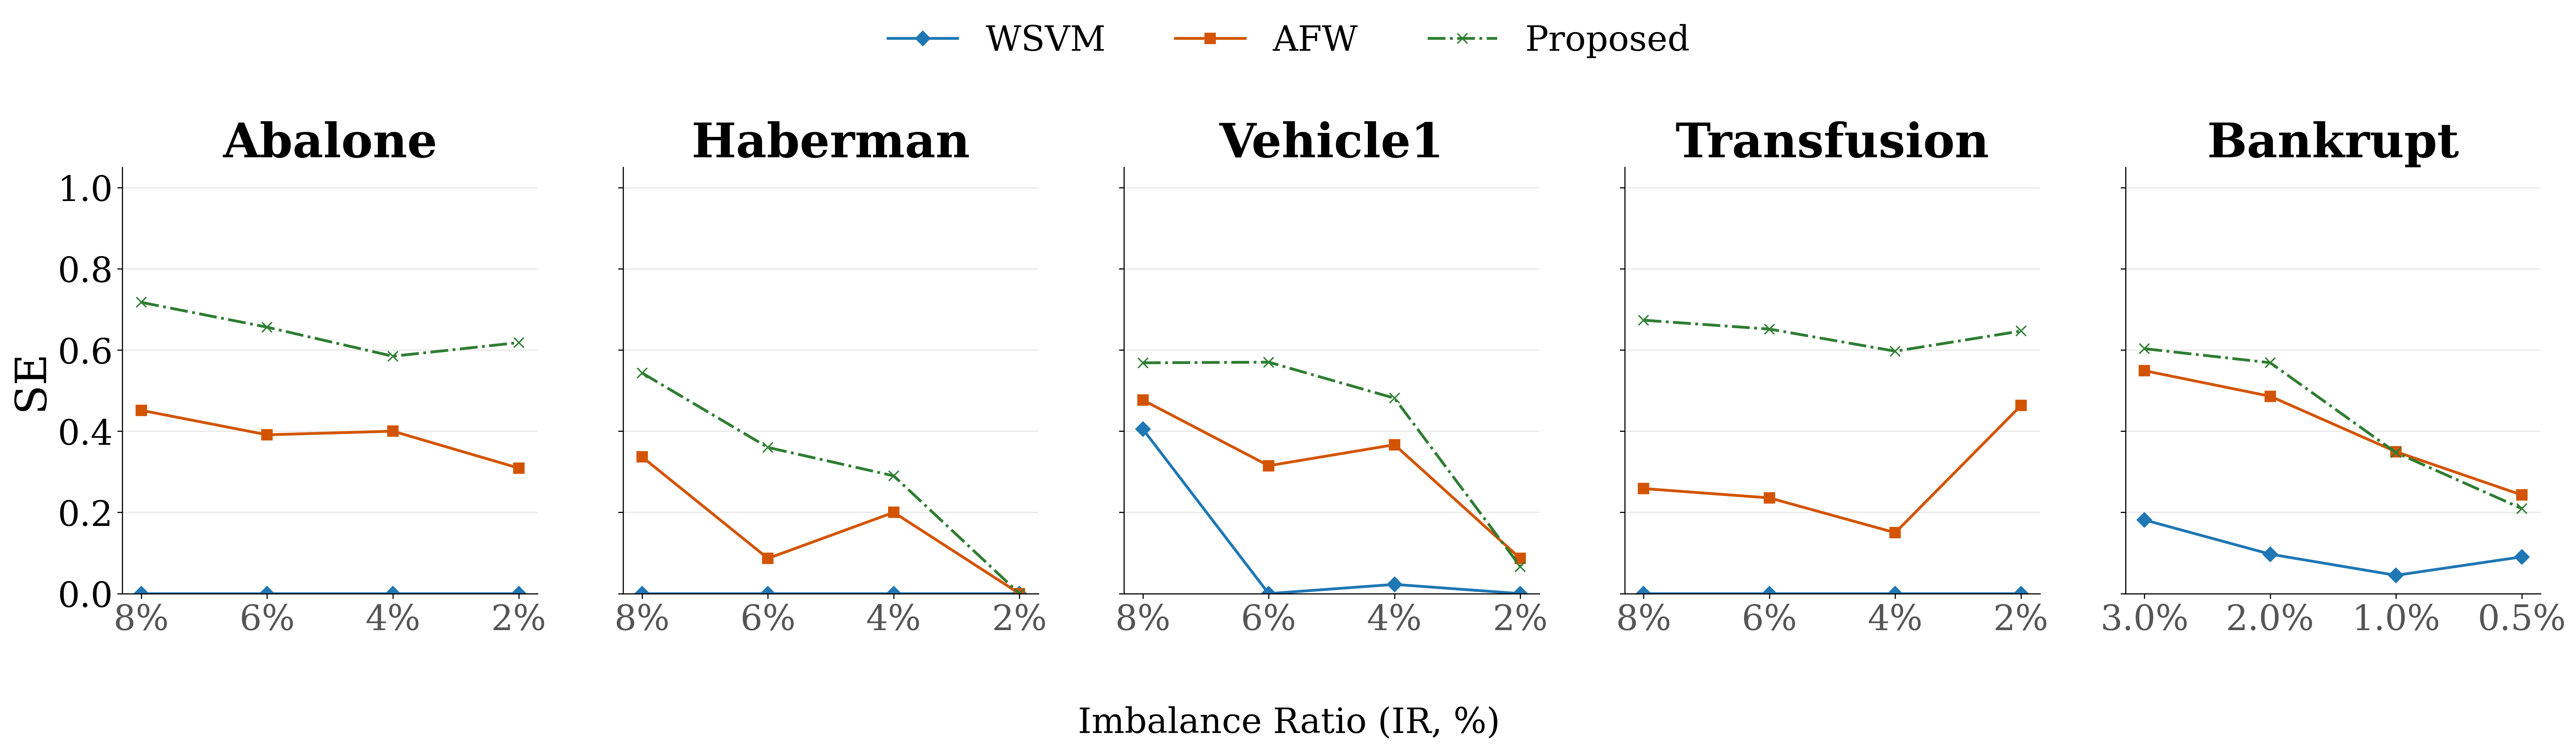
\includegraphics[width=\textwidth]{KB3_SE.png}
\caption{Performance trends in Sensitivity ($SE$) as the Imbalance Ratio (IR) decreases across the 5 representative datasets.}
\label{fig:scenario3_se}
\end{figure*}

\begin{figure*}[htbp]
\centering
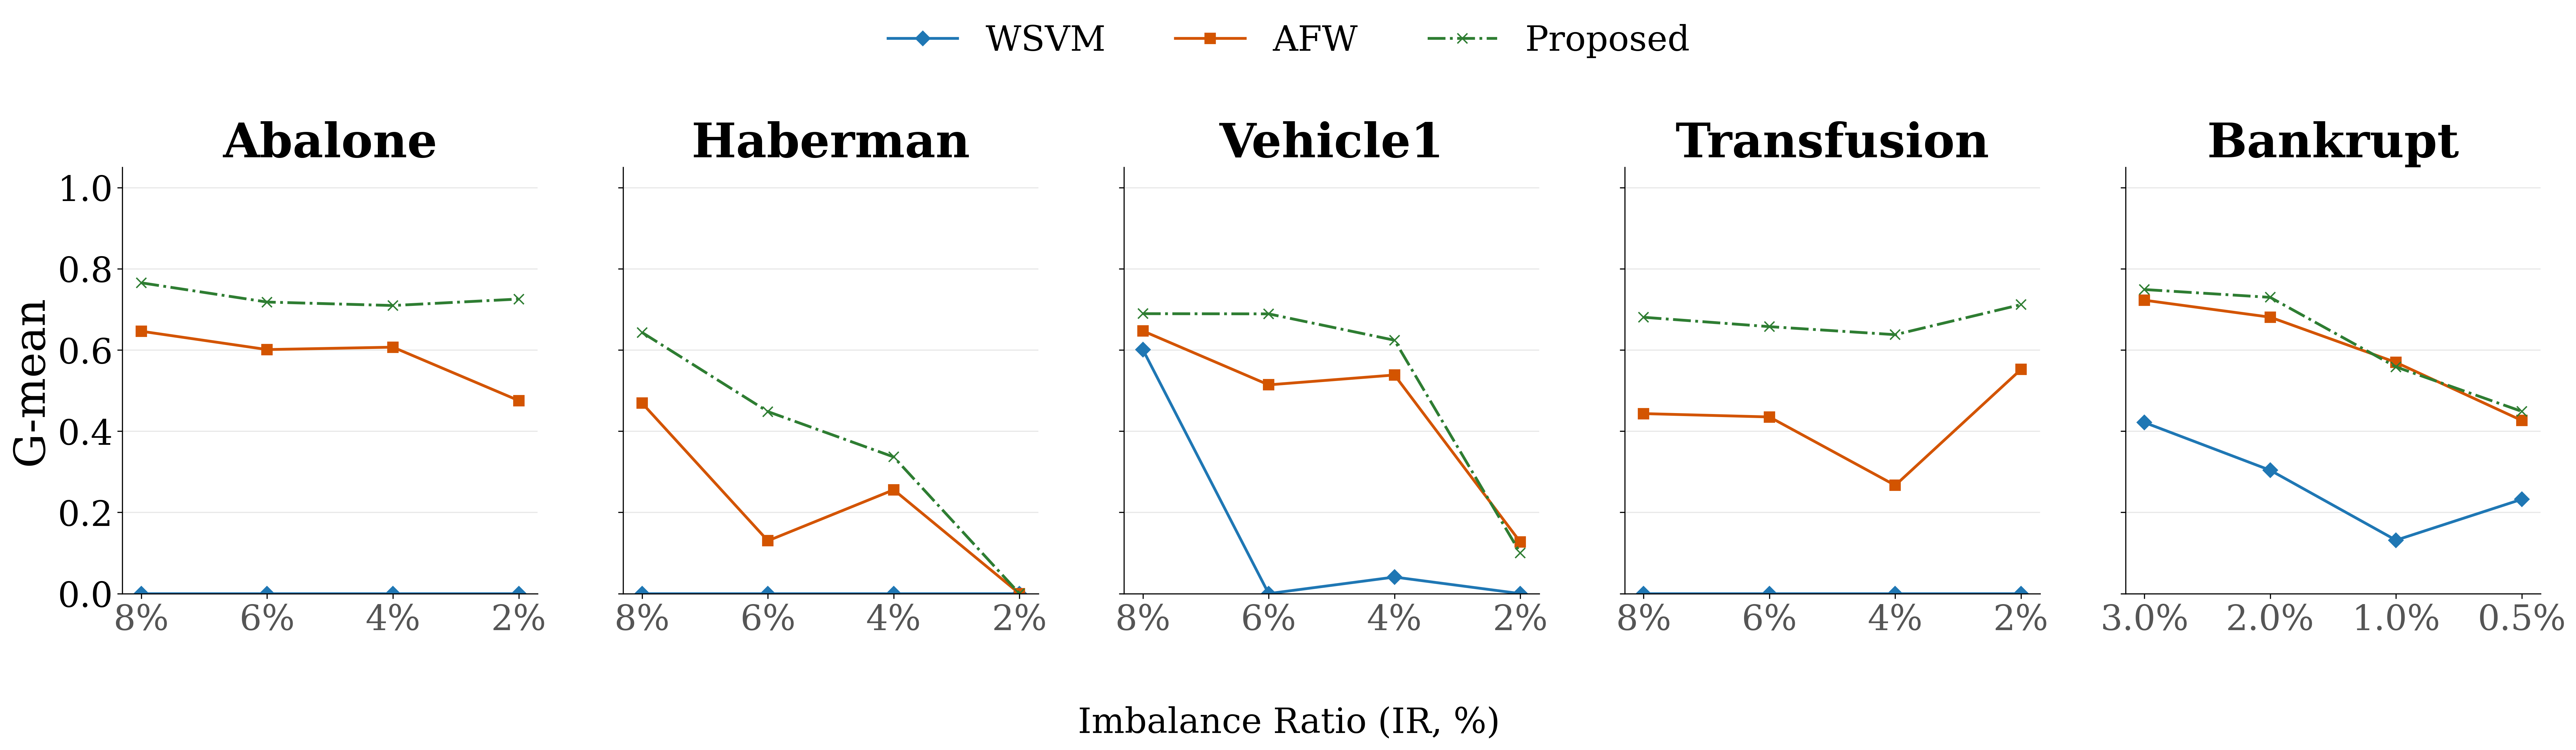
\includegraphics[width=\textwidth]{KB3_Gmean.png}
\caption{Performance trends in Geometric Mean ($Gmean$) as the Imbalance Ratio (IR) decreases across the 5 representative datasets.}
\label{fig:scenario3_gmean}
\end{figure*}

\begin{figure*}[htbp]
\centering
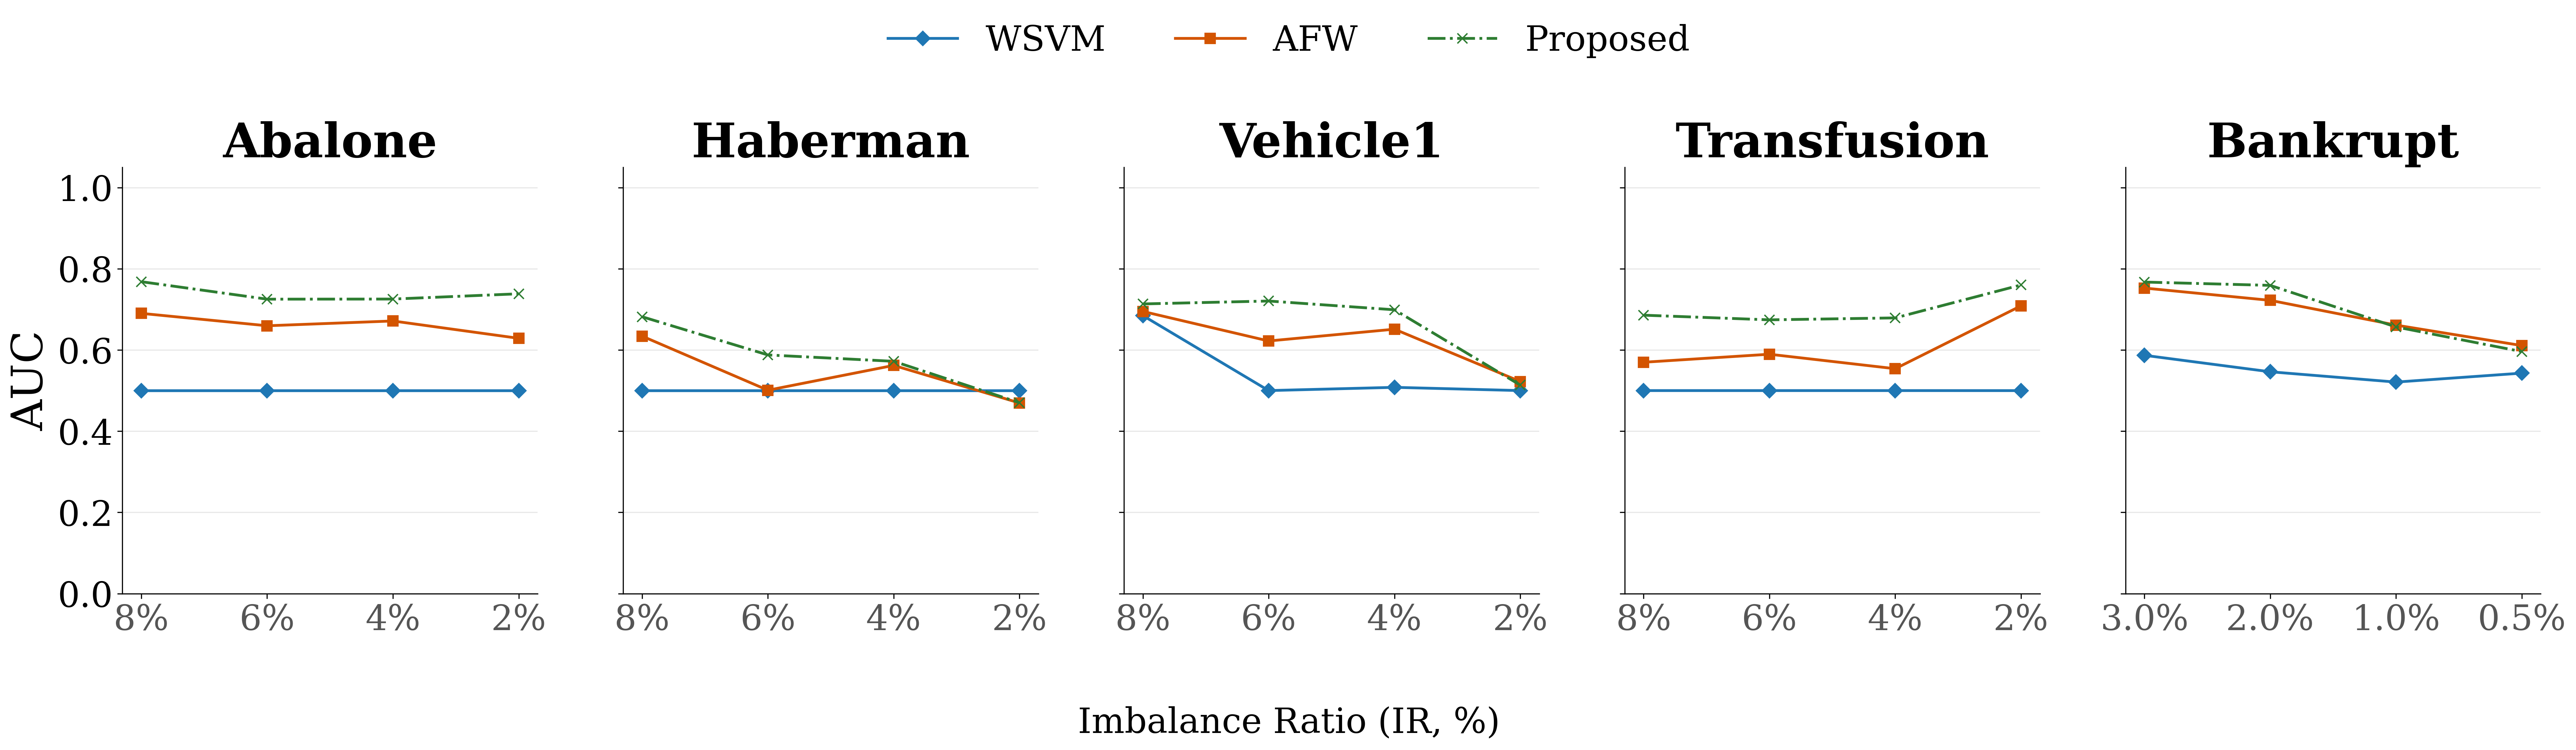
\includegraphics[width=\textwidth]{KB3_AUC.png}
\caption{Performance trends in Area Under the Curve ($AUC$) as the Imbalance Ratio (IR) decreases across the 5 representative datasets.}
\label{fig:scenario3_auc}
\end{figure*}

\smallskip
\noindent Table~\ref{tab:scenario3} and Figures~\ref{fig:scenario3_se}--\ref{fig:scenario3_auc} show the stability of the models under data scarcity. As the imbalance ratio drops toward $1\%$, the baseline W-SVM yields $SE=0.000$, and the default AFW-CIL performance decreases. In contrast, the proposed BL-SMOTE+PSO-AFW-CIL approach maintains stable $SE$, $Gmean$, and $AUC$ scores across all thresholds. Coupling BL-SMOTE with the PSO-tuned AFW-CIL core maintains accurate decision boundaries. Although this combination increases training time, it automates hyperparameter tuning and improves classification robustness.
%\pagebreak

\section{Conclusion}\label{sec5}
In this study, we propose a hybrid PSO-SMOTE approach to enhance the AFW-CIL algorithm for imbalanced data classification. The proposed approach relies on two core mechanisms: (\textit{i}) data-level oversampling, where BL-SMOTE synthesizes minority samples at borderline regions to establish accurate decision boundaries without distorting the natural data distribution; and (\textit{ii}) algorithm-level parameter tuning, where PSO automatically tunes the hyperparameters ($K, \sigma_1, \sigma_2, \sigma_3, \sigma_4$) of the AFW-CIL core. This integration eliminates manual configuration and penalizes label noise.

Experiments on 5 representative benchmark datasets show that the proposed approach improves performance over the baseline algorithms, particularly in terms of Geometric Mean ($Gmean$) and Area Under the Curve ($AUC$). It maintains stability and achieves higher Sensitivity ($SE$) under data scarcity. Although this combination increases training time, it automates hyperparameter tuning and improves classification accuracy. To mitigate this computational cost, future research could explore parallel processing techniques to accelerate the search space evaluation. Furthermore, future work will apply this approach to real-world imbalanced data tasks, such as medical diagnosis, financial fraud detection, and environmental disaster forecasting. By automating parameter selection and handling boundary noise, this approach provides a practical solution for applications where accurately identifying the minority class is critical.
\backmatter

%%======================================================================%%
%% If you are submitting to one of the Nature Portfolio journals...     %%
%%======================================================================%%

%\bibliographystyle{splncs04}

%%%\bibliography{sn-bibliography}

\begin{thebibliography}{99}

\bibitem{he2009learning}
He, H., \& Garcia, E. A. (2009). Learning from imbalanced data. \textit{IEEE Transactions on Knowledge and Data Engineering}, 21(9), 1263--1284.

\bibitem{chawla2002smote}
Chawla, N. V., Bowyer, K. W., Hall, L. O., \& Kegelmeyer, W. P. (2002). SMOTE: synthetic minority over-sampling technique. \textit{Journal of Artificial Intelligence Research}, 16, 321--357.

\bibitem{kubat1997addressing}
Kubat, M., \& Matwin, S. (1997). Addressing the curse of imbalanced training sets: one-sided selection. \textit{Proceedings of the Fourteenth International Conference on Machine Learning (ICML)}, 97(1), 179.

\bibitem{akbani2004applying}
Akbani, R., Kwek, S., \& Japkowicz, N. (2004). Applying support vector machines to imbalanced datasets. \textit{European Conference on Machine Learning}, 39--50. Springer.

\bibitem{lin2002fuzzy}
Lin, C.-F., \& Wang, S.-D. (2002). Fuzzy support vector machines. \textit{IEEE Transactions on Neural Networks}, 13(2), 464--471.

\bibitem{liu2018scalable}
Liu, J., \& Zio, E. (2018). A scalable fuzzy support vector machine for fault detection in transportation systems. \textit{Expert Systems with Applications}, 102, 36--43.

\bibitem{batuwita2010fsvm}
Batuwita, R., \& Palade, V. (2010). FSVM-CIL: fuzzy support vector machines for class imbalance learning. \textit{IEEE Transactions on Fuzzy Systems}, 18(3), 558--571.

\bibitem{quang2023adaptive}
Vo, D. Q., \& Tran, D. K. (2024). An adaptive fuzzy weight algorithm for the class imbalance learning problem. \textit{International Journal of Intelligent Information and Database Systems}. Inderscience Publishers.

\bibitem{han2005borderline}
Han, H., Wang, W.-Y., \& Mao, B.-H. (2005). Borderline-SMOTE: a new over-sampling method in imbalanced data sets learning. \textit{Proceedings of the International Conference on Intelligent Computing}, 878--887. Springer.

\bibitem{tomek1976two}
Tomek, I. (1976). Two modifications of CNN. \textit{IEEE Transactions on Systems, Man, and Cybernetics}, 6(11), 769--772.

\bibitem{kennedy1995particle}
Kennedy, J., \& Eberhart, R. (1995). Particle swarm optimization. \textit{Proceedings of ICNN'95-International Conference on Neural Networks}, 4, 1942--1948. IEEE.

\bibitem{dua2017uci}
Dua, D., \& Graff, C. (2017). UCI machine learning repository. University of California, Irvine, School of Information and Computer Sciences.

\end{thebibliography}


%% if required, the content of .bbl file can be included here
%%\input sn-article.bbl

\end{document}